\chapter{Modelling the Limit Order Book}
\label{modeling_limit_order_book}
Motivations for studying market microstructure include:
\begin{itemize}
\item \textbf{Market Simulators}: Developing market simulators to test and refine trading, market making, and execution strategies in a controlled environment before applying them to real markets.
\item \textbf{Regulatory Design}: Informing the design of relevant regulations and policies by understanding how different market structures and mechanisms impact trading behavior and market outcomes.
\item \textbf{Noise Modeling}: Creating realistic microstructure noise models to account for the inherent randomness and uncertainty in financial markets, which is crucial for accurate modeling and risk management.
\item \textbf{Price Formation}: Investigating the interplay between trading strategies and market structure in the formation of asset prices, shedding light on how trading activities influence price movements.
\item \textbf{Macro-Micro Connection}: Bridging the gap between microstructure-level analysis and macro-level variables such as market volatility, enabling a comprehensive understanding of market dynamics and their impact on broader financial conditions.
\end{itemize}
\section{The zero intelligence model (Santa Fe model)}
Several studies, including Daniels et al. (2003), Smith et al. (2003), Cont and De Larrard (2013), and Donier et al. (2015), have examined market microstructure using a common model framework. Key features of this model include:
\begin{itemize}
\item Order Book Grid: The order book is represented as a discrete price grid with a constant minimum price increment, $dp$ (the tick size).

\item Limit Order Placement: The placement of limit orders follows a Poisson process with a rate denoted as $\alpha(\Delta)$ per unit of price and unit of event time, where $\Delta$ represents the distance from the best available price.

\item Market Orders: Market orders arrive at a rate of $\mu$ per unit of event time.

\item Order Cancellations: Each existing limit order has the same probability, $\delta$, per unit of event time to be canceled.

\item Order Size: All orders, whether limit or market, have the same size, denoted as $\sigma$ shares.

\end{itemize}
This modeling approach has been found surprisingly useful in providing testable predictions for certain short-term (Cont and De Larrard, 2013) or long-term (Farmer et al., 2005) properties of the order book. Moreover, it is easy to simulate and estimate parameters from data by counting events.\\
\subsection{Asympotic depth}
Because market order arrivals only inuence activity at the best quotes, very deep into the LOB the distribution of queue sizes reaches a stationary state that is
independent of the distance from $m(t)$.\\
For $V \in \mathbb{N}$ (where $V$ is in units of the lot size $\sigma$):
\[
P_{st}(V) = e^{-V^*} \frac{(V^*)^V}{V!} \qquad V^* = \frac{\alpha}{\delta}
\]
Two extreme cases are possible:
\begin{itemize}
	\item \textbf{sparse LOB}: corrisponding to $V^* \ll 1$, where most price levels are empty, while the others are only weakly populated. This case corresponds to the behaviour of the LOB for very small-tick assets.
	\item \textbf{dense LOB}: corresponding to $V^* \gg 1$, where all price levels are populated with lagge number of orders. This corresponds to the behaviour of the LOB for large-tick assets
\end{itemize}
\subsection{Estimating the spread}
Let $S$ the spread, i.e., the difference between the best ask and bid pric, the total flux of limit orders between the mid-point and $S/2$ is $\int_0^{S/2} \alpha(\Delta) d\Delta$ where $\Delta$ is the distance from the midpoint.\\
Let us analyse better:
\begin{itemize}
	\item If $S$ is sufficiently small so that $\alpha$ is approximately costant, one finds that his incoming flux is $\sim \alpha(0)S/2$.
	\item If $\mu > \alpha(0)S/2$, the rate of market order eats up the limit orders that appear within the spread completely, and the average volume present is close to zero.
	\item If $\mu \gg \delta$, the cancellation term can be safely neglected.
	\item Argument breaks down when $S\sim 2 \mu/\alpha(0)$ which sets the typical position of the best price.
	\item The spread is therefore larger for larger market order rates, and smaller when the flow of limit order is larger, as expected intuitively.
	\item Scaling result for the spread has been derived more quantitatively when $\alpha$ and $\delta$ are indepntf od $\Delta$. One finds for the average spread:
	\[
	\expected{S} = \frac{\mu}{\alpha}F\left(\frac{\delta}{\mu}\right)
	\]
	$F(u)$ is monotonically increasing function, we can approximate it as $F(u) \sim 0.28 + 1.86u^{3/4}$
	\item In the limit where cancellation can be neglected, we obtain $S\sim 0.28 \mu / \alpha(0)$.
	\item With a similar arhuments, we show that volatility scales as:
	\[
	\expected{\sigma} \propto \mu^{5/2}\delta^{1/2}\rho^{-2}
	\]
\end{itemize}
\subsection{Dimensional analysis}
In order book we have three dimensions: price, share and time. from this we have:
\begin{itemize}
	\item Three order flow rates: Limit orders arrival rate ($\alpha$ shares/ (time$\cdot$ price)), Market order arrival rate ($\mu$ shares/time), Limit order decay ($\delta$ 1/time)
	\item Two dicreteness parameters: tocl size $dp$ (price and order size) $\sigma$ (shares)
	\item From order flows rate we derive:
	\begin{itemize}
		\item number of shares $N_c = \mu/2\delta$ 
		\item characteristic price interval $p_c = \mu / 2 \alpha$
		\item characteristic time scale $t_c = 1/ \delta$
	\end{itemize}
		\item Nondimensional scale parameter $\epsilon = \sigma/N_c$ characterizing the granularity of the orders stored in the limit-order book. A nondimensional scale parameter based on tick size is constructed by dividing by the characteristic price $dp/p_c$
		\item Continuum limit as the tick size $dp \to 0$
\end{itemize}
\begin{center}
	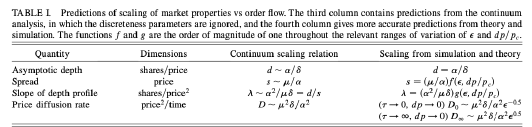
\includegraphics[width=0.6\textwidth]{picture/(24)table_dimensional_order_book.png}
\end{center}
\subsection{Model calibration}
Estimating most of the parameters in this model is expected to be quite straightforward. However, one of the model's simplifying assumptions introduces a significant challenge when fitting the model. Specifically, the model assumes that the values of $\alpha$ and $\delta$ do not vary with increasing distance from the best quotes.
To address this issue, Bouchaud et al. suggest restricting the estimation of the following parameters:
\begin{itemize}
\item $\alpha$:should be estimated only for the set $\chi_{LO}$, which includes limit orders that arrive either at the best quotes or within the spread.
\item $\delta$ : should be estimated only for the set $\chi_C$, which includes order cancellations that occur at the best quotes.
\item $\mu$:  should be estimated only for the set $\chi_{MO}$, which consists of market orders that, by definition, occur at the best quotes.
\end{itemize}
To perform these estimations, $N_{LO}, N_{C}$, and $N_{MO}$ are counted, representing the number of limit order arrivals at the best quotes, cancellations at the best quotes, and market order arrivals within a specific time window. Importantly, these counts are conducted independently of the corresponding order signs, meaning that there is symmetry between buy and sell activities.\\
The lot size $\sigma$ is estimated as:
\[
\sigma = (N_{LO})^{-1} \sum_{x \in \chi_{LO}} \sigma_{\chi}
\]
where $\sigma_{\chi}$ is the size (in shares) of LOs.\\
The total MO arrival rate per event $2\tilde{\mu}$ is estimates as:
\[
\tilde{\mu} = (N_{MO} + N_{LO} + N_C)^{-1} \sum_{\chi \in \chi_{MO}} (\sigma_x/\sigma)
\]
The total limit order arrival rate per event is:
\[
2\tilde{\alpha}_{all} = \frac{N_{LO}}{N_{MO} + N_{LO} + N_{C}}
\]
The limit order arrival rate in the ZI model is a rate per unit price, so to estimate $\tilde{\alpha}$
we divide $\tilde{\alpha}_{all}$ all by the mean number $n$ of available price levels inside the spread and
at the best quotes, measured only at the times of limit order arrivals.\\
The total cancellation rate per unit volume and per event is\footnote{Note that the above estimation procedures all lead to rates per event rather than rates per unit time.}:
\[
2\tilde{\delta} = \frac{1}{N_{MO} + N_{LO} + N_{C}}\sum_{x \in \chi_C} \frac{\sigma_x}{\bar{V}} \qquad \bar{V} = \frac{\bar{V}_a + \bar{V}_b}{2}
\]
From Bouchauad et all, we estimated parameters: $\tilde{\lambda} \to \tilde{\alpha}, \tilde{\nu} \to \tilde{\delta}, v_0 \to \sigma$.\\
One of the limits is the presence of arbitrage opportunities
\[
\mathcal{R}_\tau \equiv \expected{\epsilon_t (m_{t +\tau} - m_t)} \simeq \frac{1}{2} P (V_{best} = v_0)\expected{\text{first gap}}
\]
\begin{myquote}
This simple observation has an important consequence: the Santa Fe model specification leads to profitable market-making strategies, even when the signature plot is flat (i.e. when prices are diffusive). $[\ldots]$ market-making is profitable on average if the mean bid-ask spread is larger than twice the long-term impact $\mathcal{R}_{\infty}$. In the Santa Fevmodel, the mean first gap is always smaller than the bid-ask spread. Therefore, $R_{\infty} < \expected{\text{spread}}=2$, so market-making is easy within this framework."
\end{myquote}
The cancellation rate depends on past volatility:
\[
\delta_t = \delta + a_k \left(\int_0^t \sqrt{2 \beta} e^{-\beta(t-s)}dP_s\right)^2
\]
Spread abruptly increases because of the feedback
\section{Heavy traffic limit: Cont and de Larrad (2013)}
For most liquid stocks, where both market orders and limit orders arrive at a high rate, the imbalance between limit orders (which increase the queue size) and market orders and cancellations (which decrease the queue size) is typically much smaller in magnitude. In this scenario, limit orders accumulate and disappear at same rate. Consequently, the behavior of the order queues follows a diffusive pattern, making it pertinent to consider the diffusion limit of the limit order book (similar brownian motion).\\
In the diffusion limit, the rescaled order book process for the two queues converges weakly to a Brownian motion in the positive orthant $\{x \geq 0, y \geq 0\}$ represent the volume at the best ask and best bid, respectively. These volumes are refreshed when the "walker" reaches one of the two axes, indicating queue depletion.\\
The probability that the next price move is an increase, given a queue of x shares on the bid side and y shares on the ask side, can be expressed as:
\[
p_{up}(x,y) = \frac{1}{2} - \frac{\arctan\left(\sqrt{\frac{1+\rho}{1-\rho}} \frac{y-x}{y+x}\right)}{2 \arctan\left(\sqrt{\frac{1+ \rho}{1- \rho}}\right)}
\]
where $\rho$ is the correlation between order sizes at the bid and at the ask
\newpage
\section{Latent Limit Order Book}
In modern electronic markets traders interact through a limit order book (LOB) in a continuous double auction.
\begin{itemize}
	\item Continuous refers to time: at each moment traders can take an action on the LOB
	\item Double auction means that the LOB is divided into two sides: bid side (buyers) + ask side (sellers)
\end{itemize}
\begin{center}
	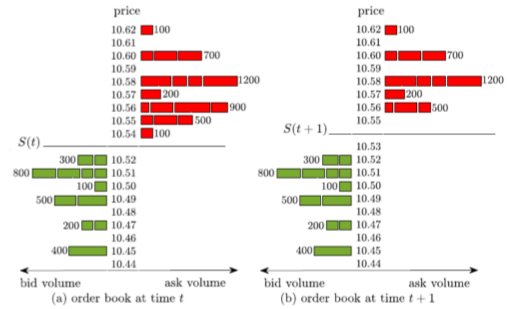
\includegraphics[width=0.5\textwidth]{picture/(25)snapshot_lob.png}
\end{center}
Let give some remarks:
\begin{itemize}
	\item weak instantaneous liquidity ($< 1 \%$ of daily traded volume)
	\item The revealed LOB is short lived.
	\item Since the square-root impact law is an aggregate low-frequency phenomenon, the relevant object to consider cannot be the revealed LOB
\end{itemize}
Most of the available liquidity is latent and it is only progressively reveales during the day (like mealting tip of an iceberg).\\
MM only act as small intermediaries between the much larger volume imbalances of low frequency actors that can only get resolved on large time scales.
\subsection{Latent Limit Order Book scheme}
\begin{enumerate}
	\item The trade intentions are stored in the latent limit order book (LLOB)
\begin{center}
	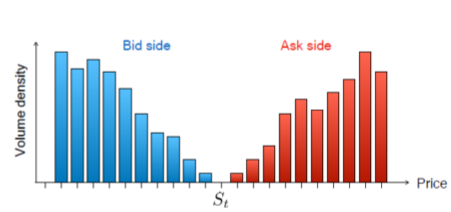
\includegraphics[width=0.5\textwidth]{picture/(26)lob_1.png}
\end{center}
\item The trade intentions are stored in the latent limit order book (LLOB in dark color) and may or not materialise in the revealed limit order book (LOB in lighter color). Latent orders are revealed in the vicinity od the trade price $S_t$. No incentive i giving away private information too soon!
\begin{center}
	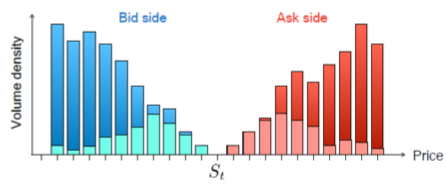
\includegraphics[width=0.5\textwidth]{picture/(27)lob_2.png}
\end{center}
\end{enumerate}
\subsection{Simple Geometrical Considerations}
Let consider a static world:\\
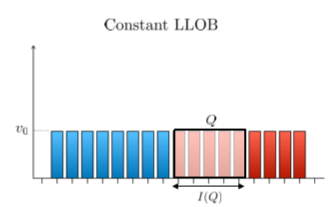
\includegraphics[width=0.35\textwidth]{picture/(28)costant_llob.png}\\
$Q = I(Q) \times v_0 \rightarrow I(Q) =Q/v_0$ linear market impact.\\
Let consider now a linear LLOB:\\
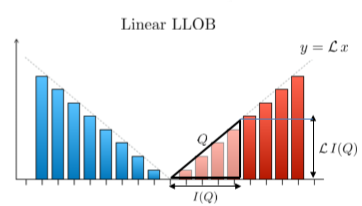
\includegraphics[width=0.35\textwidth]{picture/(29)linear_llob.png}\\
$ Q = (I(Q) \times \mathcal{L} I(Q))/2 \rightarrow I(Q) = \sqrt{2Q\mathcal{L}}$ square root market impact\\
This model is not realistic, we need to include dynamics.
\subsection{Coarse Grained Dynamics}
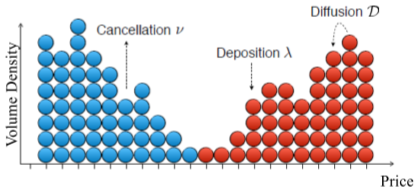
\includegraphics[width=0.3\textwidth]{picture/(30)react_diff_1.png} $\Rightarrow$ 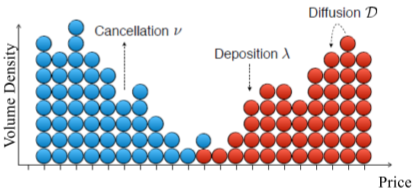
\includegraphics[width=0.3\textwidth]{picture/(31)react_diff_2.png}  $\Rightarrow$ 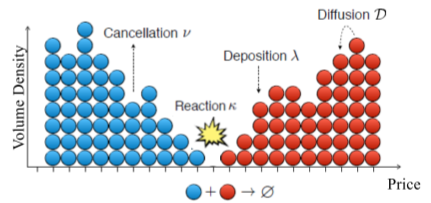
\includegraphics[width=0.3\textwidth]{picture/(32)react_diff_3.png}\\
A first dynamical approach has been proposed by J. Donier et al (Quantitaive Finance 2015):
\begin{center}
	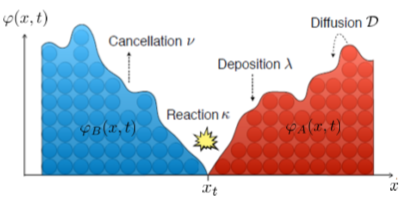
\includegraphics[width=0.5\textwidth]{picture/(33)coarse_grained_dynamics.png}
\end{center}
\begin{align*}
	&\partial_t \varphi_A(x,t) = \mathcal{D} \partial_{xx} \varphi_A(x,t) - \nu \varphi_A(x,t) + \lambda \Theta(x_t -x) - R_{A,B}(x,t)\\
	&\partial_t \varphi_B (x,t) = \underbrace{\mathcal{D} \partial_{xx} \varphi_B(x,t)}_{\text{Diffusion}} - \underbrace{\nu \varphi_B(x,t)}_{\text{Cancellation}} + \underbrace{ \lambda \Theta(x_t -x)}_{\text{Deposition}} - \underbrace{R_{A,B}(x,t)}_{\text{Reaction}}
\end{align*}
where $R_{A,B}(x,t) = \kappa \varphi_a(x,t) \varphi_B(x,t)$. The price equation for the transaction price $x_t$ is:
\[
\varphi_a(x_t,t) = \varphi_B (x_t,t)
\]
Some consideration:
\begin{itemize}
	\item in the limit $\kappa \to \infty$ no overlap between $\varphi_A, \varphi_B$
	\item reaction-diffusion problem in solvable considering the difference:
	\begin{align*}
		&\varphi(x,t):= \varphi_B(x,t) - \varphi_A(x,t)\\
		&\partial_t \varphi(x,t) = \mathcal{D}\partial_{xx} \varphi(x,t) - \nu \varphi(x,t) + \lambda \text{sign}(x_t-x)
	\end{align*}
with boundary conditions:
\begin{align*}
	&\varphi(x_t,t) = 0 \quad \forall t\\
	&\lim_{|x| \to \infty} \varphi(x,t) \neq \infty\\
	&\varphi(x, t=0) = -\varphi(-x, t = 0)
\end{align*}
with $\varphi(x, t=0)$ the initial symmetric state of latent order book
\end{itemize}
We can evaluate the stationaruy LLOB solving:
\[
\partial_t \varphi^{st}(\xi,t) = 0 \rightarrow \mathcal{D}\partial_{xx} \varphi^{st}(\xi) - \nu \varphi^{st}(\xi) = \lambda
\]
with $\xi = x - S_t$, we get:
\[
\varphi^{st}(\xi) = -\frac{\lambda}{\nu} \text{sign}(\xi)(1- e^{-|\xi|/\xi_c})
\]
where $\xi_c := \sqrt{\mathcal{D}/\nu}$ and the market total turnover equal to:
\[
J:= \mathcal{D}\partial_\xi \varphi^{st}|_{\xi = 0} = \mathcal{D}\mathcal{L}
\]
\begin{center}
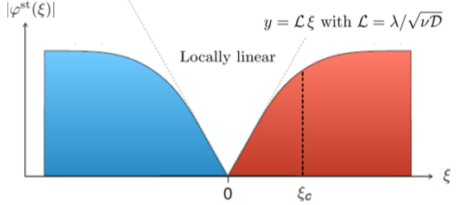
\includegraphics[width=0.4\textwidth]{picture/(34)stationary_llob.png}
\end{center}
Let evaluate the market impact: first of all Let us assume to execute the metaorder with volume:
\[
Q =\int_0^T m(\tau)d(\tau) \qquad m(\tau) = \text{trading intensity rate} 
\]
Following Donier et al approach, in the infinit memory limit $\nu,\lambda \to 0$ with constant $\mathcal{L} \sim \lambda \nu^{-1/2}$, so the price dynamics is given solving:
\[
\partial_t \varphi(x,t) = \mathcal{D}\partial_{xx} \varphi(x,t) + m(t)\delta(x-x_t)
\]
(the last one is the extra current of buy/sell particles falling at the transition price $x =x_t$), with the boundary conditions:
\begin{align*}
	&\varphi(x,t = 0) = \varphi^{\text{st}}(x)\\
	&\lim_{x \to \infty} \partial_x \varphi(x,t) = -\mathcal{L}
\end{align*}
Imposing $\varphi(x_t,t) =0$ in the solution of the PDE:
\[
\varphi(x,t) = - \mathcal{L}x + \int_0^t d\tau \frac{m(\tau)}{\sqrt{4\pi\mathcal{D}(t-\tau)}}e^{-\frac{(x-x_\tau)^2}{4\mathcal{D}(t-\tau)}}
\]
we obtain the following self-consistent relation for the transaction pric:
\[
x_t = \frac{1}{\mathcal{L}}\int_0^t d\tau \frac{m(\tau)}{\sqrt{4\pi\mathcal{D}(t-\tau)}}e^{-\frac{(x-x_\tau)^2}{4\mathcal{D}(t-\tau)}}
\]
If impact is small $|y(s)-y(t)|^2 \ll D(t-s)$ the price dybamics becomes:
\[
y(t) = \frac{1}{\mathcal{L}} \int_0^t \frac{ds m(s)}{\sqrt{4 \pi D(t-s)}}
\]
This makes explicit the fact that in this model market impact is transient!\\
In general the equation for $x_t$ can be solved numerically and the price impact $I:=x_T$ is described by:
\[
I(Q) = \frac{\mathcal{D}Q}{J} \mathcal{F}(\eta)
\]
with $\eta = Q/(JT)$ the participation rate and:
\[
\mathcal{F} \sim 
\begin{cases}
\sqrt{\eta/\pi} & \text{for } \eta \ll 1 \quad \text{small participation rate}\\
\sqrt{2} & \text{for } \eta \gg 1 \quad \text{large participation rate}
\end{cases}
\]
It follows that in the infinite memory LLOB model the market impact $I(Q)$:
\begin{itemize}
	\item is linear in $Q$ for small $Q$ at fixed $T$
	\item crosses over to a square root for large $Q$
	\item is independent from $T$ in the square root regime
\end{itemize}
\begin{center}
	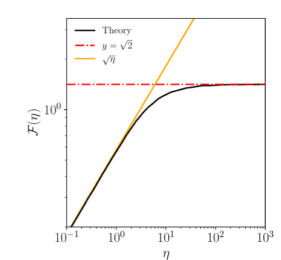
\includegraphics[width=0.4\textwidth]{picture/(35)solution_llob.png}
\end{center}
Estimate it with empirical data:
\begin{center}
	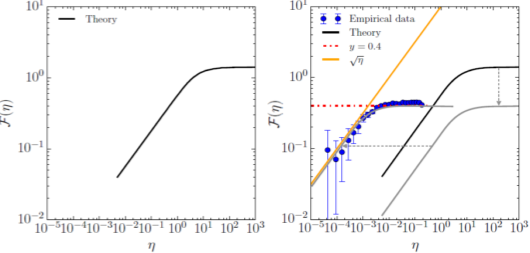
\includegraphics[width=0.4\textwidth]{picture/(36)empirical_data_llob.png}
\end{center}
We noticed that there is a good qualitative afreement but not quantitative.\\
The intuition is that the total market turnover $J$ is actually dominated by HFTs/MM, while resistance to show metaorders can only be provided by slow participants(institutional investors). For this reason we introduce the LLOB model with two time-scales for market participants: fast and slow ones.\\
We consider slow agent:$\lambda_s, \nu_s$ and fast agents: $\lambda_f,\nu_f$ with $\lambda_s,\nu_s \ll \lambda_f,\nu_f$/\\
Two contributions to the latent order book:
\begin{align*}
	&\partial_t \varphi_s(x,t) = \mathcal{D}_s \partial_{xx} \varphi_s(x,t) - \nu_s \varphi_s(x,t) + \lambda_s(x_t -x) \quad \text{with } \nu_sT \to 0 \quad \text{(infinite memory)}\\
	&\partial_t \varphi_f(x,t) = \mathcal{D}_f \partial_{xx} \varphi_f(x,t) - \nu_f \varphi_f(x,t) + \lambda_f(x_t -x) \quad \text{with } \nu_fT \gg 1 \quad \text{(very short memory)}
\end{align*}
Let $\xi = x -x_t$, the total market turnover is:
\[
J = |\mathcal{D}_s \partial_\xi \varphi_s^{st} + \mathcal{D}_t\partial_\xi \varphi_f^{st}|_{\xi =0} =J_s +J_f \quad \text{with } J_f \gg J_s\to J \sim J_f
\]
We focus on two different regime, where the metaorder intensity $m_0$ is:
\begin{itemize}
	\item large compared to the average transaction rate of slow traders $J_s$ (long time)\\
	\item but small compared to the total transaction rate of the market $J$ (short time)
	\[
	J_s \ll m_0 \ll J
	\]
\end{itemize}
We modify the equation including this information:
\begin{align*}
	&\partial_t \varphi_s(x,t) = \mathcal{D}_s \partial_{xx} \varphi_s(x,t) - \nu_s \varphi_s(x,t) + \lambda_s(x_t -x) + m_{s,t}\delta(x-x_t)\\
	&\partial_t \varphi_f(x,t) = \mathcal{D}_f \partial_{xx} \varphi_f(x,t) - \nu_f \varphi_f(x,t) + \lambda_f(x_t -x) + m_{f,t} \delta(x-x_t)
\end{align*}
with $m_{f,t} + m_{s,t} =m_0 \quad \forall t$ (we added the fraction of the metaorder executed against the slow liquidity and the metaorder executed against the fast liquidity).\\
Price equation is
\[
\varphi(x_t,t) = \varphi_s(x_t,t) + \varphi_f(x_t,t) = 0
\]
We can solve this model for $T > T^\dag$ where:
\begin{itemize}
	\item $T^\dag = \nu_f^{-1}\eta^{*-2}\mathcal{D}_s/\mathcal{D}_f$
	\item $\eta^* = J_s/J_f$
For $T > T^\dagger$ the price impact is described by the scaling:
\[
I(Q) = \sqrt{\frac{\mathcal{D}_sQ}{J_s}}\mathcal{F}\left(\frac{\eta}{\eta^*}\right)
\]
\end{itemize}
We can recover the infinite memory LLOB rescaling both the axis:
\[
I(Q) = \sqrt{\frac{\mathcal{D}Q}{J}} \mathcal{F}(\eta) \xrightarrow[]{\sqrt{\frac{\mathcal{D}_sQ}{\mathcal{D}J_s}}}\sqrt{\frac{\mathcal{D}_sQ}{\mathcal{D}J_s}} \mathcal{F}(\eta)\xrightarrow[]{\eta \to \frac{\eta}{\eta^*}} \sqrt{\frac{\mathcal{D}_sQ}{J_s}} \mathcal{F}\left(\frac{\eta}{\eta^*}\right)
\]
\begin{center}
	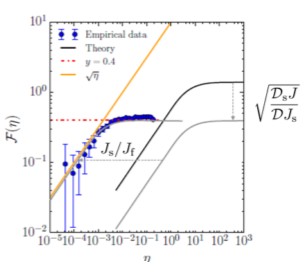
\includegraphics[width=0.4\textwidth]{picture/(37)fast_slow_llob.png}
\end{center}
Allowing at least two characteristic timescales for the liquidity (fast and slow) we empirically confirm the crossover from a linear to a square to a square root regime described by:
\[
I(Q) \propto \sqrt{Q} \mathcal{F}(\eta)\sim \begin{cases}
	Q & \text{for } \eta \ll \eta^* \quad \text{'small participation rate regime'}\\
	\sqrt{Q} & \text{for } \eta \gg \eta^* \quad \text{'large participation rate regime'}
\end{cases}
\]
with $\eta = Q/(JT)$, $T =t_{end} - t_{start}$ and:
\[
\mathcal{F}(\eta) \sim \begin{cases}
	\sqrt{\eta/\pi} & \eta \ll \eta^*\\
	c = 0.4 & \eta \ll \eta^*
\end{cases}
\]
Market impact should not be misconstrued as volatility, in particular the square root law has nothing to do with price diffusion, price changed $\Delta s$ grow as the square root of duration $\sqrt{T}$.\\
Let give some final comments:
\begin{itemize}
	\item In agreement with dynamical liquidity (earlier equation) the market impact is characterized by a crossover from a linear to a square root regime
	\item The market impact in the square-root regime is independent drom the execution duration $T$
	\item Market impact should not be misconstrued as volatility
\end{itemize}
\section{Queue-reactive order book model} 
In their paper "Simulating and analyzing order book data: The queue-reactive model," Huang, W., Lehalle, C.A., and Rosenbaum, M. (2015) introduce three models for simulating the dynamics of the limit order book (LOB). Their central idea is that order flow still follows a Poissonian process, but the arrival rate is contingent on the current state of the LOB. As the order flow influences and modifies the state of the LOB, this interaction leads to order flow that is both auto-correlated (correlated with itself over time) and cross-correlated (correlated with other order flow components).
\begin{mysetting}[Queue-reactive order book]
	\begin{itemize}
		\item The LOB is modeled as a $2K-$dimensional process, $X(t) = \{q_{-k}(t,\ldots, q_{-1}(t),q_1(t),\ldots,q_k(t))\}$, where $q_i(t)$ is the number of shares at price level $i$ (ticks) from the reference price $p_{ref}$
		\item $p_{ref}$ is equal to the midprice when the spread is equal to one tick or an odd number of ticks. When it is even, it is either:
		\[
		p_{mid} + \frac{\text{tick}}{2}\qquad \text{or }\qquad p_{mid} - \frac{\text{tick}}{2}
		\]
		choosing the one which is the closest to the privious valure of $p_{ref}$
		\item The arrival rates $\lambda_L^i (X(t)), \lambda_C^i (X(t))$, and $\lambda^i_M (X(t))$ of limit, cancellation and market order, respectively, at level $i \in \{-K,\ldots, K\}$, depend on:
		\begin{itemize}
			\item only of the target queue size (Model 1)
			\item also of the size of the other queues (Model 2)
			\item also the most recent chanfe in the reference price (Model 3)
		\end{itemize}
	\end{itemize}
\end{mysetting}
$n_{tot}$ shares must be executed in $M$ periods. In each period we want to trade $n_i$ shares.\\
While optimal execution (e.g Almgren-Chriss) tells us how much to trade in each period, it is silent about how to trade (e.g. limit vs market orders, when to cancel, etc) in each period. In the $i$th slice, both tactics post a limit order of size $n_i$ at the best offer queue at the beginning of the period, and send a market order with all the remaining quantity to complete the execution of the target volume at the end time of the slice. In between:
\begin{itemize}
	\item T1 (Fire and forget): When $p_{mid}$ changes, cancel the limit order and send a market order at the opposite side with all the remaining volume if any.
	\item T2 (Pegging to the best): When the best offer price changes or our order is the only remaining orser at the best offer limit, cancel the order and repost all the remaining volume at the newly revealed best offer queue
\end{itemize}
Two types of order scheduling strategies:
\begin{itemize}
	\item S1: A linear scheduling ($n_i = n_{tot}/M)$, used for the VWAP benchmark
	\item S2: An exponential scheduling $n_i = n_{tot} (e^{-(i-1)/4} - e^{-i/4})$ with the arrival price $S_0$ as benchmark
\end{itemize}
\begin{center}
	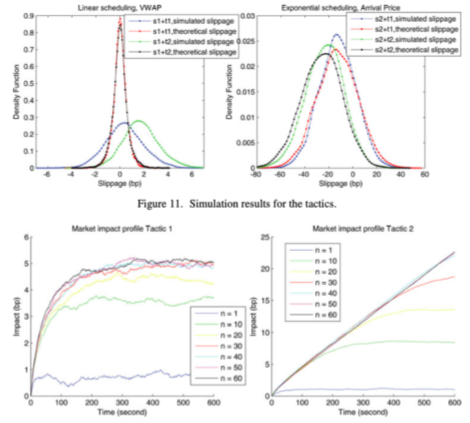
\includegraphics[width=0.5\textwidth]{picture/(38)order_placement_analysis.png}
\end{center}

